\documentclass[main.tex]{subfiles}
\begin{document}
\begin{bmcsex}{Pullout with piecewise linear bond-slip law}{e32_pullout_multilinear}
\noindent The pull-out response is calculated for specifying the values 
    explicitly specified bond-slip law.
 \\
\begin{center}
            
{\scriptsize 
\begin{longtable}{lrp{4cm}}\toprule
\textbf{\textsf{Model parameter}} 
& 
\textbf{\textsf{Symbol = Value [Unit]}} 
&
\textbf{\textsf{Description}}  \\\midrule \midrule
\texttt{k\_max} & $k_{\max}$ = 1000 [$\mathrm{mm}$] & {\footnotesize maximum number of iterations}  \\
            \texttt{fixed\_boundary} & None = non-loaded end (matrix) [None] & {\footnotesize which side of the specimen is fixed}  \\
            \texttt{u\_f0\_max} & $u_{\mathrm{f},0,{\max}}$ = 1.84 [mm] & {\footnotesize maximum displacement of the pulled reinforcement}  \\
            \texttt{mats\_eval\_type} & None = multilinear [None] & {\footnotesize material model type}  \\
            \texttt{tolerance} & $\epsilon$ = 0.0001 [-] & {\footnotesize tolerance of residual}  \\
            \texttt{n\_e\_x} & $n_\mathrm{E}$ = 100 [-] & {\footnotesize number of finite elements along the embedded length}  \\
            \midrule
\multicolumn{3}{l}{\textbf{\textsf{Geometry: geometry}}}\\

\texttt{geometry.L\_x} & $L$ = 200.0 [$\mathrm{mm}$] & {\footnotesize embedded length}  \\
            \midrule
\multicolumn{3}{l}{\textbf{\textsf{CrossSection: cross\_section}}}\\

\texttt{cross\_section.A\_f} & $A_\mathrm{f}$ = 16.67 [$\mathrm{mm}^2$] & {\footnotesize reinforcement area}  \\
            \texttt{cross\_section.A\_m} & $A_\mathrm{m}$ = 1540.0 [$\mathrm{mm}^2$] & {\footnotesize matrix area}  \\
            \texttt{cross\_section.P\_b} & $P_\mathrm{b}$ = 1.0 [$\mathrm{mm}$] & {\footnotesize perimeter of the bond interface}  \\
            \midrule
\multicolumn{3}{l}{\textbf{\textsf{MATSBondSlipMultiLinear: mats\_eval}}}\\

\texttt{mats\_eval.s\_data} & $s$ = 0, 0.1, 0.4, 4.0 [mm] & {\footnotesize slip values}  \\
            \texttt{mats\_eval.tau\_data} & $\tau$ = 0, 800, 0, 0 [MPa] & {\footnotesize shear stress values}  \\
            \texttt{mats\_eval.E\_f} & $E_\mathrm{f}$ = 170000.0 [MPa] & {\footnotesize E-modulus of the reinforcement}  \\
            \texttt{mats\_eval.E\_m} & $E_\mathrm{m}$ = 28000.0 [MPa] & {\footnotesize E-modulus of the matrix}  \\
            
\multicolumn{3}{r}{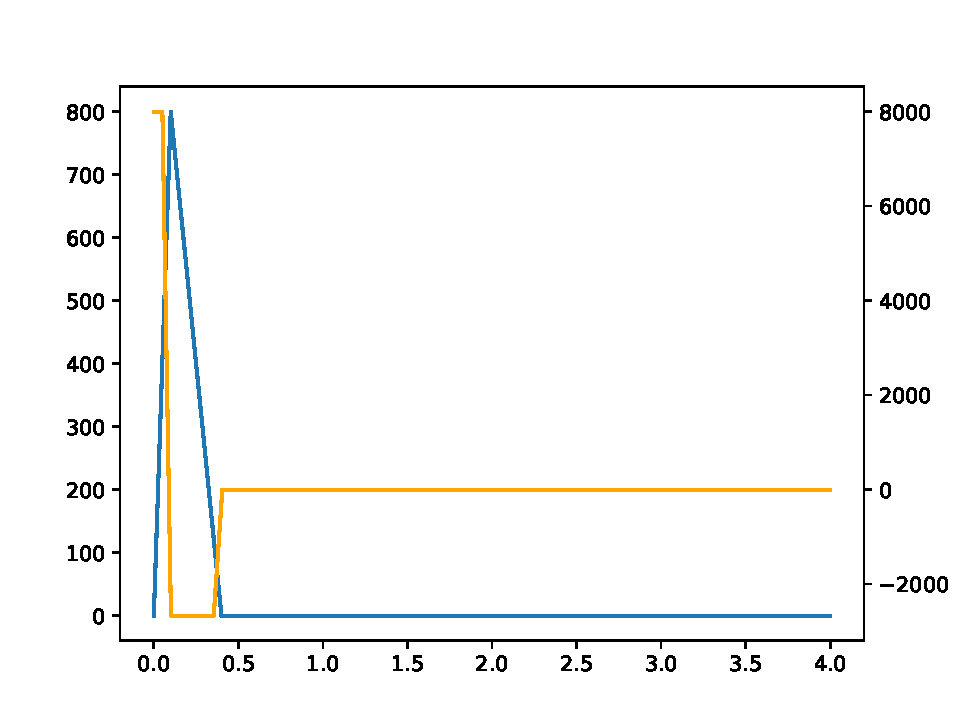
\includegraphics[width=5cm]{examples/e32_pullout_multilinear/fig_multilinear_bond_law.pdf}}\\
\bottomrule 
\end{longtable}
}

    Loading is applied at the right end of the specimen. The specimen
    is fixed at the unloaded end by prescribing zero matrix displacement. 
    Four stages of loading are displayed as marked in the
    loading scenario and in the pull-out curve.
    \begin{longtable}{c}
\mbox{
    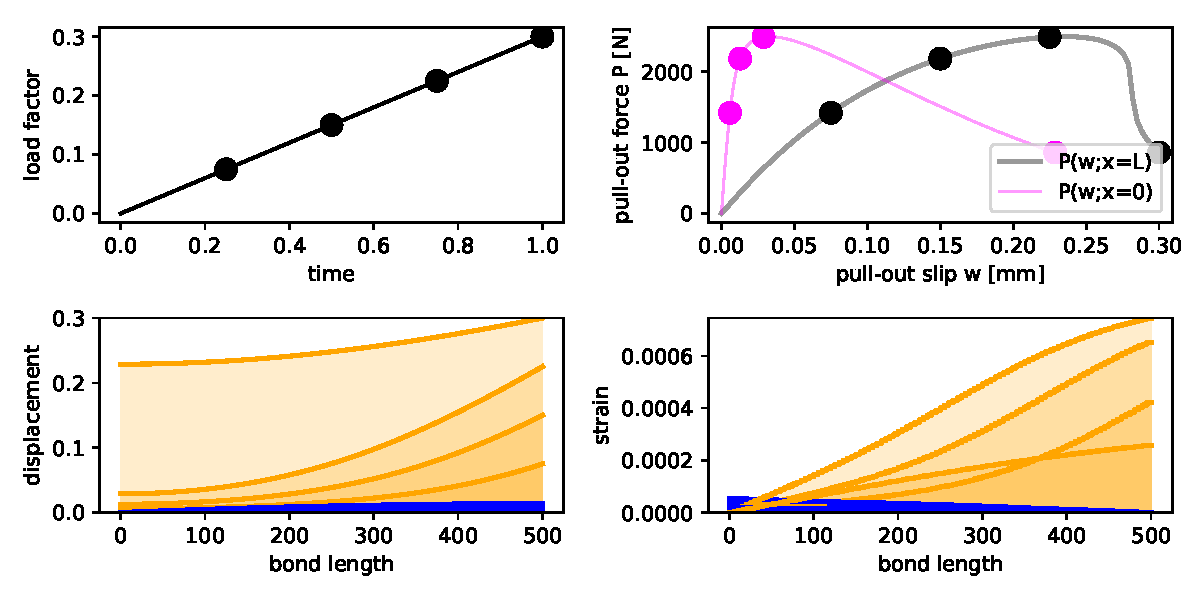
\includegraphics[width=0.8\textwidth]{examples/e32_pullout_multilinear/fig_frictional_bond01.pdf}
    }\\
    
    \mbox{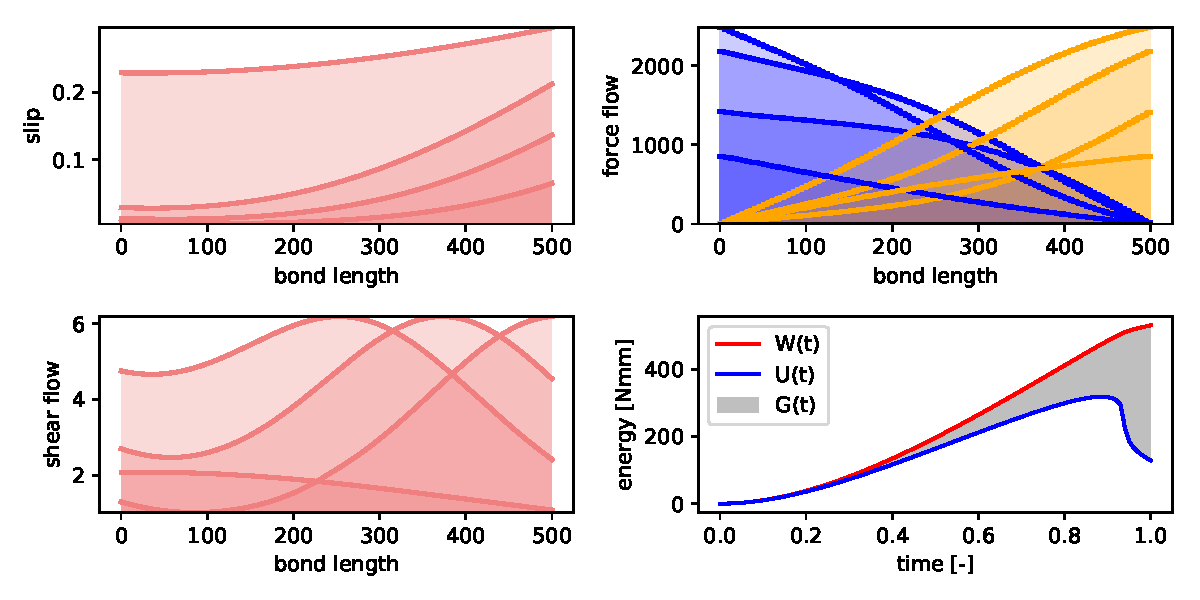
\includegraphics[width=0.8\textwidth]{examples/e32_pullout_multilinear/fig_frictional_bond02.pdf}}

    
    \end{longtable}
    \end{center}
            \end{bmcsex}
\end{document}
    